%% 
%% Copyright 2007-2020 Elsevier Ltd
%% 
%% This file is part of the 'Elsarticle Bundle'.
%% ---------------------------------------------
%% 
%% It may be distributed under the conditions of the LaTeX Project Public
%% License, either version 1.2 of this license or (at your option) any
%% later version.  The latest version of this license is in
%%    http://www.latex-project.org/lppl.txt
%% and version 1.2 or later is part of all distributions of LaTeX
%% version 1999/12/01 or later.
%% 
%% The list of all files belonging to the 'Elsarticle Bundle' is
%% given in the file `manifest.txt'.
%% 

%% Template article for Elsevier's document class `elsarticle'
%% with numbered style bibliographic references
%% SP 2008/03/01
%%
%% 
%%
%% $Id: elsarticle-template-num.tex 190 2020-11-23 11:12:32Z rishi $
%%
%%
\documentclass[preprint,12pt]{elsarticle}

%% Use the option review to obtain double line spacing
%% \documentclass[authoryear,preprint,review,12pt]{elsarticle}

%% Use the options 1p,twocolumn; 3p; 3p,twocolumn; 5p; or 5p,twocolumn
%% for a journal layout:
%% \documentclass[final,1p,times]{elsarticle}
%% \documentclass[final,1p,times,twocolumn]{elsarticle}
%% \documentclass[final,3p,times]{elsarticle}
%% \documentclass[final,3p,times,twocolumn]{elsarticle}
%% \documentclass[final,5p,times]{elsarticle}
%% \documentclass[final,5p,times,twocolumn]{elsarticle}

\usepackage[margin=0.5in]{geometry}

%% For including figures, graphicx.sty has been loaded in
%% elsarticle.cls. If you prefer to use the old commands
%% please give \usepackage{epsfig}
\usepackage{graphicx}

%% The amssymb package provides various useful mathematical symbols
\usepackage{amssymb}
%% The amsthm package provides extended theorem environments
%% \usepackage{amsthm}

%% The lineno packages adds line numbers. Start line numbering with
%% \begin{linenumbers}, end it with \end{linenumbers}. Or switch it on
%% for the whole article with \linenumbers.
%% \usepackage{lineno}

\journal{Applied Catalysis B}

\begin{document}

\begin{frontmatter}

\title{Hydrogen Adsorption Energy Necessary but Not Sufficient for HER Catalysis: Connecting Machine-Learned Descriptors with High-Throughput Experimental Catalysis over Bimetallic Nanoparticles}

\author[add1]{Kirby Broderick}
\author[add2]{Eric Lopato}
\author[add1]{Brook Wander}

\author[add2]{Stefan Bernhard}
\author[add1]{John Kitchin}
\author[add1]{Zachary Ulissi*}
\ead{zulissi@andrew.cmu.edu}
\address[add1]{Carnegie Mellon University Department of Chemical Engineering, 5000 Forbes Avenue, Pittsburgh PA 15213, USA}
\address[add2]{Carnegie Mellon University Department of Chemistry, 4400 Fifth Avenue, Pittsburgh PA 15213, USA}

\raggedright
\begin{abstract}
  The Sabatier principle is of fundamental importance to computational catalyst discovery, saving researchers time and expense by predicting catalytic activity \emph{in silico} at scale. However, as polycrystalline and nanoscale catalysts increasingly dominate industry, computational screening tools must be adapted to these uses. In this work, we demonstrate the effectiveness of computational adsorption energy screening in nanocatalysis by comparing a multisite adsorption energy prediction workflow against a large experimental dataset of hydrogen evolution activities over bimetallic nanoparticles. Comparing 16 million hydrogen adsorption energy predictions with the hydrogen evolution activity of 5,300 experiments across 84 monometallic and bimetallic systems, we discover that favorable adsorption energies are a necessary condition for experimental activity, but other factors often determine trends in practice. About half of the bimetallic search space can be excluded from experimental screens using hydrogen adsorption predictions, but these tools may become significantly more powerful when combined with other screening tools.
\end{abstract}

\begin{keyword}
%% keywords here, in the form: keyword \sep keyword
Hydrogen Evolution Reaction \sep computational catalysis \sep Sabatier principle \sep high-throughput screening \sep nanocatalysis
\end{keyword}

\end{frontmatter}

%% \linenumbersjust

%% main text
\raggedright
\section{Introduction}

The discovery of new catalysts for fundamental reactions such as water splitting, ammonia synthesis, or CO$_2$ reduction is a fundamental to the development of an environmentally sustainable economy. By increasing reaction efficiency, catalysts offer the possibility of reducing industrial energy requirements and enabling more sustainable chemical production processes \cite{osti_1545774}. However, the space of all possible catalysts is too vast to be surveyed experimentally \cite{tran2018active}. For this reason, the field of computational catalysis tries to predict catalytic activity using materials properties. One important tool is the Sabatier principle, which describes a volcano-shaped relationship between the binding energy of a key reaction specie and the overall reaction rate \cite{medford2015Sabatier}. Although this relationship was developed using experimental binding energies \cite{trasatti1972work}, these values can be computed using Density Functional Theory (DFT), a computationally tractable approximation to quantum chemistry \cite{osti_1545774,ooka2021sabatier}.

Modern efforts to computationally screen chemical composition space for new catalysts began almost two decades ago. N{\o}rskov et al. \cite{norskov2005trends} established a kinetic model that uses DFT-calculated $\Delta$E(*H) on an fcc site to predict exchange current density. This work also considered the effects of changing coverage and found them to be minimal. Later efforts by the same group looked at multiple adsorption sites in more detail, screening bimetallic alloys modeled as a pure metal with a secondary metal incorporated into the surface layer \cite{greeley2006computational} and further developing the kinetic model \cite{skulason2010modeling} (see Figure 1). The latter work used 1 monolayer coverage for all materials on the left half of the volcano. The researchers also made the observation that, despite the fact that many of the metals on the left-hand side of the volcano should be oxidized, experimental values align with adsorption calculations made using metallic surfaces. 

\begin{figure}[h]
\centering
    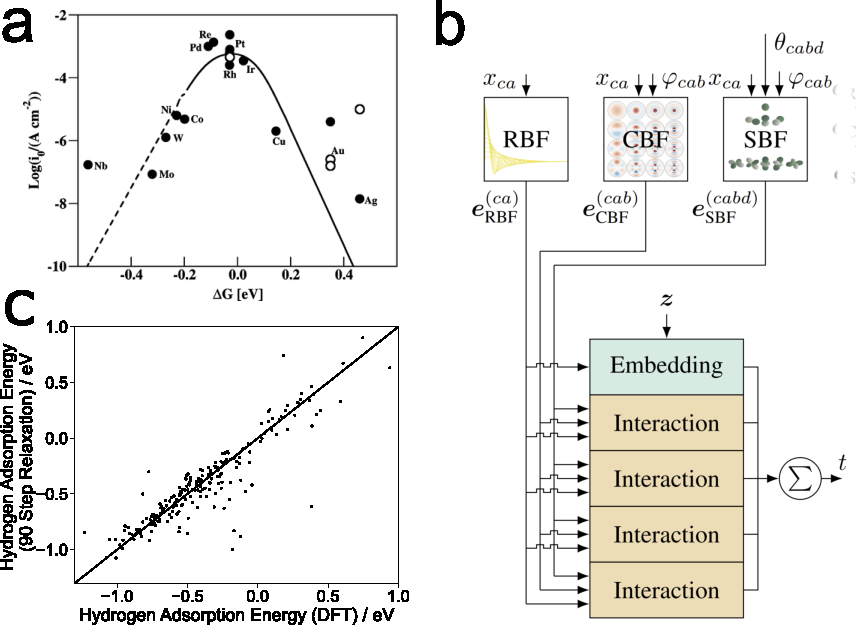
\includegraphics[width=0.6\textwidth]{figures/fig_1.pdf}
\caption{(a) A volcano plot for hydrogen evolution taken from Skúlason et al. \cite{skulason2010modeling}. Measured exchange current density is plotted against the free energy of hydrogen adsorption at U=0V. Adsorption energies were calculated using DFT, assuming 0.25 monolayer coverage for metals on the right-hand side of the volcano, and 1 monolayer coverage otherwise. The kinetic model is represented as a line; the dashed line represents the expectation that metals this strong binding will oxidize. (b) A block diagram detailing the structure of GemNet, the message-passing graph neural network used in this work to model DFT hydrogen adsorption energies, taken from Klicpera et al. \cite{klicpera2021gemnet}. These adsorption energies are used to construct the x-axis of the volcano plot used in this work. (c) A parity plot comparing the predicted hydrogen adsorption energy after a 90-step relaxation using the model depicted in (b) to DFT validation data. This demonstrates the accuracy of the machine learned model (MAE = 0.1 eV).}
\end{figure}

The development of computationally grounded volcano plots has spurred researchers to find ways to optimize and streamline their use in catalytic discovery. Tran and Ulissi (2018) established a high-throughput automated screening method using active learning to discover materials with binding energies that indicate activity for hydrogen evolution and CO$_2$ reduction \cite{tran2018active}. Another effort established a data set of DFT calculations and associated community challenges to spur interest in machine learning models capable of approximating DFT adsorption energies across a variety of adsorbates and materials for catalyst discovery \cite{chanussot2021open}. 

 However, several complications differentiate industrial catalysts from the slab models commonly used to compute adsorption energies \cite{norskov2005trends,tran2018active}. Modern industrial catalysts are often highly nanostructured, experiencing size-specific chemical phenomena that impact catalysis \cite{khorshidi2018strain}, and nanoparticles may undergo surface or bulk segregation to form a distribution of structures and surfaces in practice \cite{mitchell2021nanoscale,vallee2001size}. Furthermore, it is not always clear which surfaces and binding sites are most responsible for catalytic activity, which is confounded by the difficulty of experimentally characterizing structure or surface expression at the scale of modern computational and experimental screens \cite{yang2022applications}. Bimetallic nanoparticles have been of interest for their catalytic properties for many reactions in recent decades \cite{toshima1998bimetallic,singh2013synergistic}. The expanded bimetallic material search space offers the possibility of discovering cheaper or more active catalysts while remaining tractable using modern computational techniques \cite{tran2018active}.
 
 
In previous work, we developed a high-throughput method for synthesizing bimetallic nanoparticles and measuring their ability to catalyze the Hydrogen Evolution Reaction (HER) \cite{lopato2020parallelized,bhat2022accelerated,simon2022ligand}. In this procedure, metal salts are combined with a photocatalyst, and light stimulates the reduction of ions into nanoparticles and the subsequent evolution of hydrogen gas (see Fig. 2). In this work, we assess the sufficiency of hydrogen adsorption energy predictions in describing the resulting data: the experimental HER activities of bimetallic nanoparticles are compared with a computational workflow that predicts and aggregates hydrogen adsorption energies across various surfaces from intermetallic crystal structures from the Materials Project \cite{ong2013python}. Our computational workflow is distinguished from previous efforts because it automates the process of predicting adsorption energies across different binding sites, surfaces, and materials, allowing catalysis experiment and theory to be compared at greater scales than previously possible.

\section{Experimental}\label{Section:Experimental}
\subsection{High-throughput Synthesis and Assay of Bimetallic Nanoparticles}
To explore the expanse of bimetallic space for in situ nanoparticle synthesis, the concentration of two different precursor salts were varied in each column and row of a high-throughput photoreactor. Each vial comprised [Ir(Fmppy)$_2$dtbbpy]PF$_6$ photosensitizer at 0.25 mM concentration, 400 $\mu$L of DMSO (J.T. Baker JT9224), 40 $\mathrm{\mu}$L of a 30 percent (w/w) aqueous TEOA (Alfa Aesar L04486) solution, and metal salts at concentrations varying between 0.05 and 0.65 $\mathrm{\mu}$M. Experiments included the metals Ag, Al, Au, Bi, Co, Cr, Eu, Fe, Ga, In, Ir, La, Li, Mn, Mo, Ni, Os, Pb, Pd, Pt, Rh, Ru, Sn, V, and Zn. A list of metal salt precursors is given in the Supporting Information.

Reaction wells were illuminated over blue LEDs in a parallelized reactor setup as described previously. Using colorimetric chemosensitive H$_2$ detection tape (DetecTape Hydrogen Detection Tape-Midsun Specialty Products, Item DT-H210015-PF4), the reactions were tracked in real-time using image analysis to reveal the quantity of hydrogen produced by each. Calibrations for this method can be found in our previous work \cite{lopato2020parallelized}.


\subsection{Computational Enumeration and Prediction of Sites}\label{Section:Experimental/Enumeration}
Starting with the dataset of intermetallic Materials Project structures created from bulks with nonpositive formation energies at most 0.1 eV above hull enumerated in the Open Catalyst Dataset \cite{chanussot2021open,ong2013python}, slabs were enumerated using Open Catalyst Dataset enumeration tools, and CatKit was used to position adsorption sites over the surfaces \cite{boes2019graph}. All bare structures larger than 80 atoms and all slabs larger than 100 atoms were discarded due to computational constraints, representing less than 1\% of structures and approximately 30\% of slabs. Hydrogen adsorption energies of the adsorbate-slab systems were then calculated using GemNet, a graph neural network that uses message passing with directed edge embeddings to predict materials properties from structures \cite{klicpera2021gemnet}. The model had been trained on the Open Catalyst Dataset and is available on the Open Catalyst Project website \cite{chanussot2021open}. Systems were relaxed for 90 steps, a procedure which accurately predicts validation data (see Figure 1). After adsorption energies were predicted, the minimum (strongest) adsorption energy was taken to represent the surface. 


\subsection{Formation of Volcano Plot}\label{Section:Experimental/Volcano}
For every metal system (e.g. Au-Ni), corresponding surface minimum adsorption energies were selected from the calculated adsorption energy data set based on whether the corresponding structure had a bulk electrochemical stability below 0.5 eV/atom as calculated using the Materials Project PourbaixDiagram module \cite{singh2017electrochemical,persson2012prediction,patel2019efficient}, assuming a pH of 8.5, a voltage of -1.2 V \cite{lowry2005single}, and every metal ion at a concentration of 0.6 mM (corresponding approximately to the upper end of experimental metal ion concentration). The minimum hydrogen binding energy on every facet was taken, then the value closest to -0.24 eV (representing approximate thermodynamic neutrality after free energy correction \cite{norskov2005trends}) was chosen to represent the overall binding energy of the chemical system. Experimental activities were calculated by smoothing observed cumulative hydrogen evolution over time with a Gaussian filter and taking the maximum rate for every trial (see Figure 2). After averaging experimental values observed under identical input conditions, we used the maximum rate across every experiment within a metal system to represent chemical activity (see Fig. 3). 

\begin{figure}[h]
\centering
    \includegraphics[width=0.9\textwidth]{figures/fig_2.pdf}
\caption{(a) An image of an experimental well plate during a hydrogen evolution experiment. Darkening of the wells over time corresponds to hydrogen adsorption onto a chemosensory tape, which is then used to determine cumulative hydrogen evolution. (b) The underside of a well plate during an experiment. (c) The proposed catalytic cycle for hydrogen evolution observed in experiments in this work \cite{lopato2020parallelized}. The photosensitizer is charged by a sacrificial oxidant and then reduces a catalyst, resulting in the formation of hydrogen from water. (d) Time series data for the cumulative evolution of hydrogen over time for a single well in an experiment. The slope of the red line denotes the maximum rate observed. This maximum rate is aggregated across multiple experiments with the same metal combination and the resulting value is used in place of exchange current density as the y-axis of our volcano plot. (e) The observed maximum HER rates for various experiments containing only Au metal salt. Rates from experiments that ran concurrently in different wells are plotted using the same color and shape. Rates were averaged across all experiments that used the same metal salts at the same concentrations (average values are depicted as black bars), and the highest average rate is used to represent the metal system on the volcano plot.
}
\end{figure}

\begin{figure}[H]
\centering
    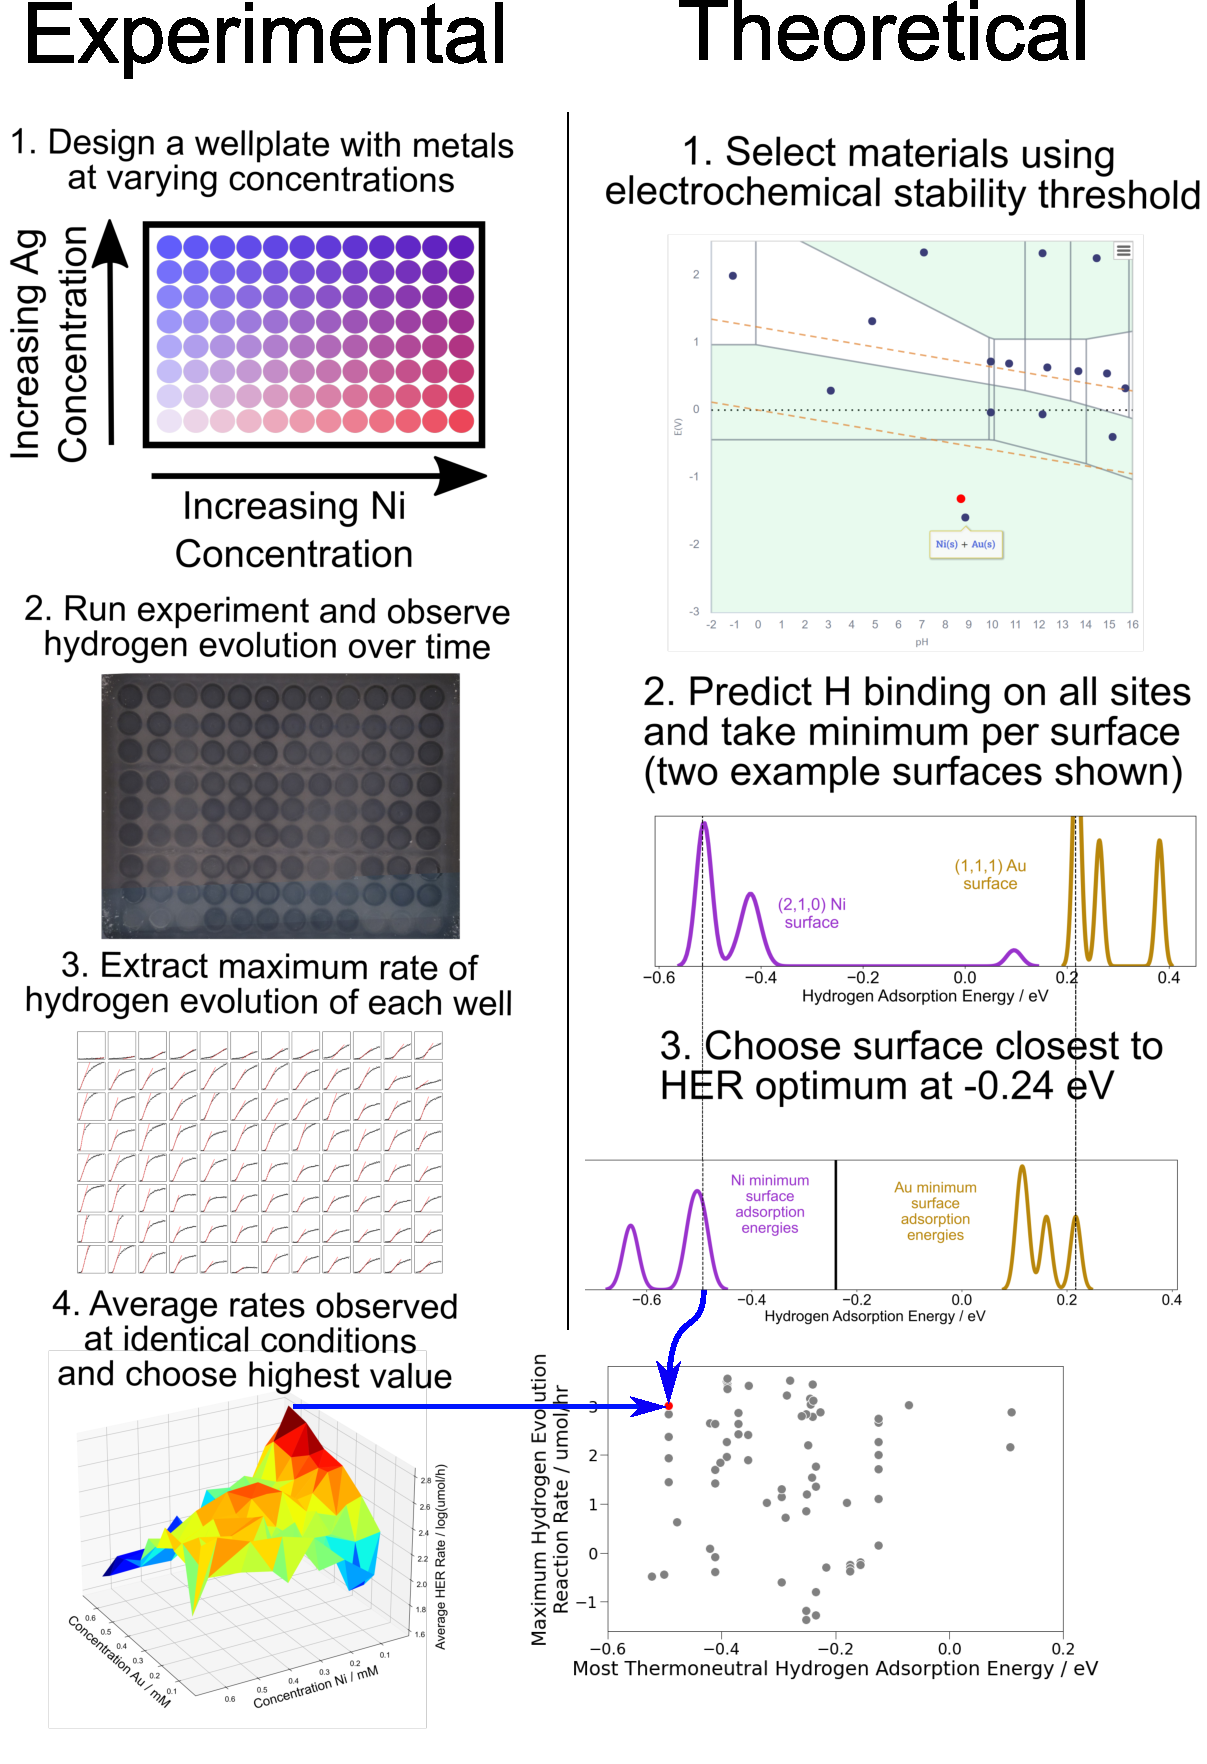
\includegraphics[width=0.6\textwidth]{figures/fig_3.pdf}
\caption{A schematic detailing the formation of the volcano plot for the example of the gold-nickel system. (left) The y-axis of the volcano plot is constructed using a set of experiments conducted in the same chemical system (top left; a single well plate is shown). For each experiment, the maximum rate of change over time is determined after smoothing (center left), and then experiments conducted at the same conditions are averaged to create a map of maximum rate as a function of composition (bottom left). The highest value is then used to represent the reaction rate of the chemical system on the volcano plot (bottom right). (right) The x-axis of the volcano plot is constructed starting with crystal structures taken from the Materials Project. A Pourbaix Diagram is used to find stable crystals at representative chemical conditions (top right). Then, hydrogen adsorption energy predictions are made for enumerated sites, and the lowest value is taken for every surface on each crystal (two representative surfaces chosen). The surface closest to -0.24 eV is used to represent the chemical system on the x-axis of the volcano plot (bottom right).
}
\end{figure}

\section{Results and discussion}\label{Section:Results}
\subsection{Aggregating hydrogen binding energies across a chemical system}
A single physical descriptor cannot capture the dynamics of such a complex process as {\it in situ} nanoparticle formation and catalysis, and uncertainty in the physical process makes it difficult to predict the outcome of individual trials directly without fine control of process conditions. Accurate and comprehensive models of nanoparticle formation, growth, or surface expression remain elusive, and current works typically use experimental characterization techniques to model small numbers of systems in detail \cite{chen2019kinetics,ma2019toward,gamler2019achieving}, although some multisystem screening tools have been developed recently \cite{wahl2021machine,li2019intermetallic,palizhati2019toward}. Experimental binding energies also often differ significantly from theoretical values, which are generally calculated using DFT over low-index intermetallic surfaces. Such complications include coverage effects \cite{frey2014implications}, surface poisoning and passivation \cite{quaino2014volcano}, transport limitations \cite{rheinlander2013comparing}, and surface strain \cite{khorshidi2018strain}. The HER over a platinum surface, one of the fastest chemical reactions ever observed, appears to progress through a weak-binding adsorbed intermediate \cite{lindgren2019challenge,ooka2021non}. However, other sources argue that in spite of these factors, the Sabatier principle can be used as a heuristic to guide experimenters toward a subset of materials with the potential for activity \cite{ulissi2011effect,schipper2018effects}. 

\begin{figure}[h]
\centering
    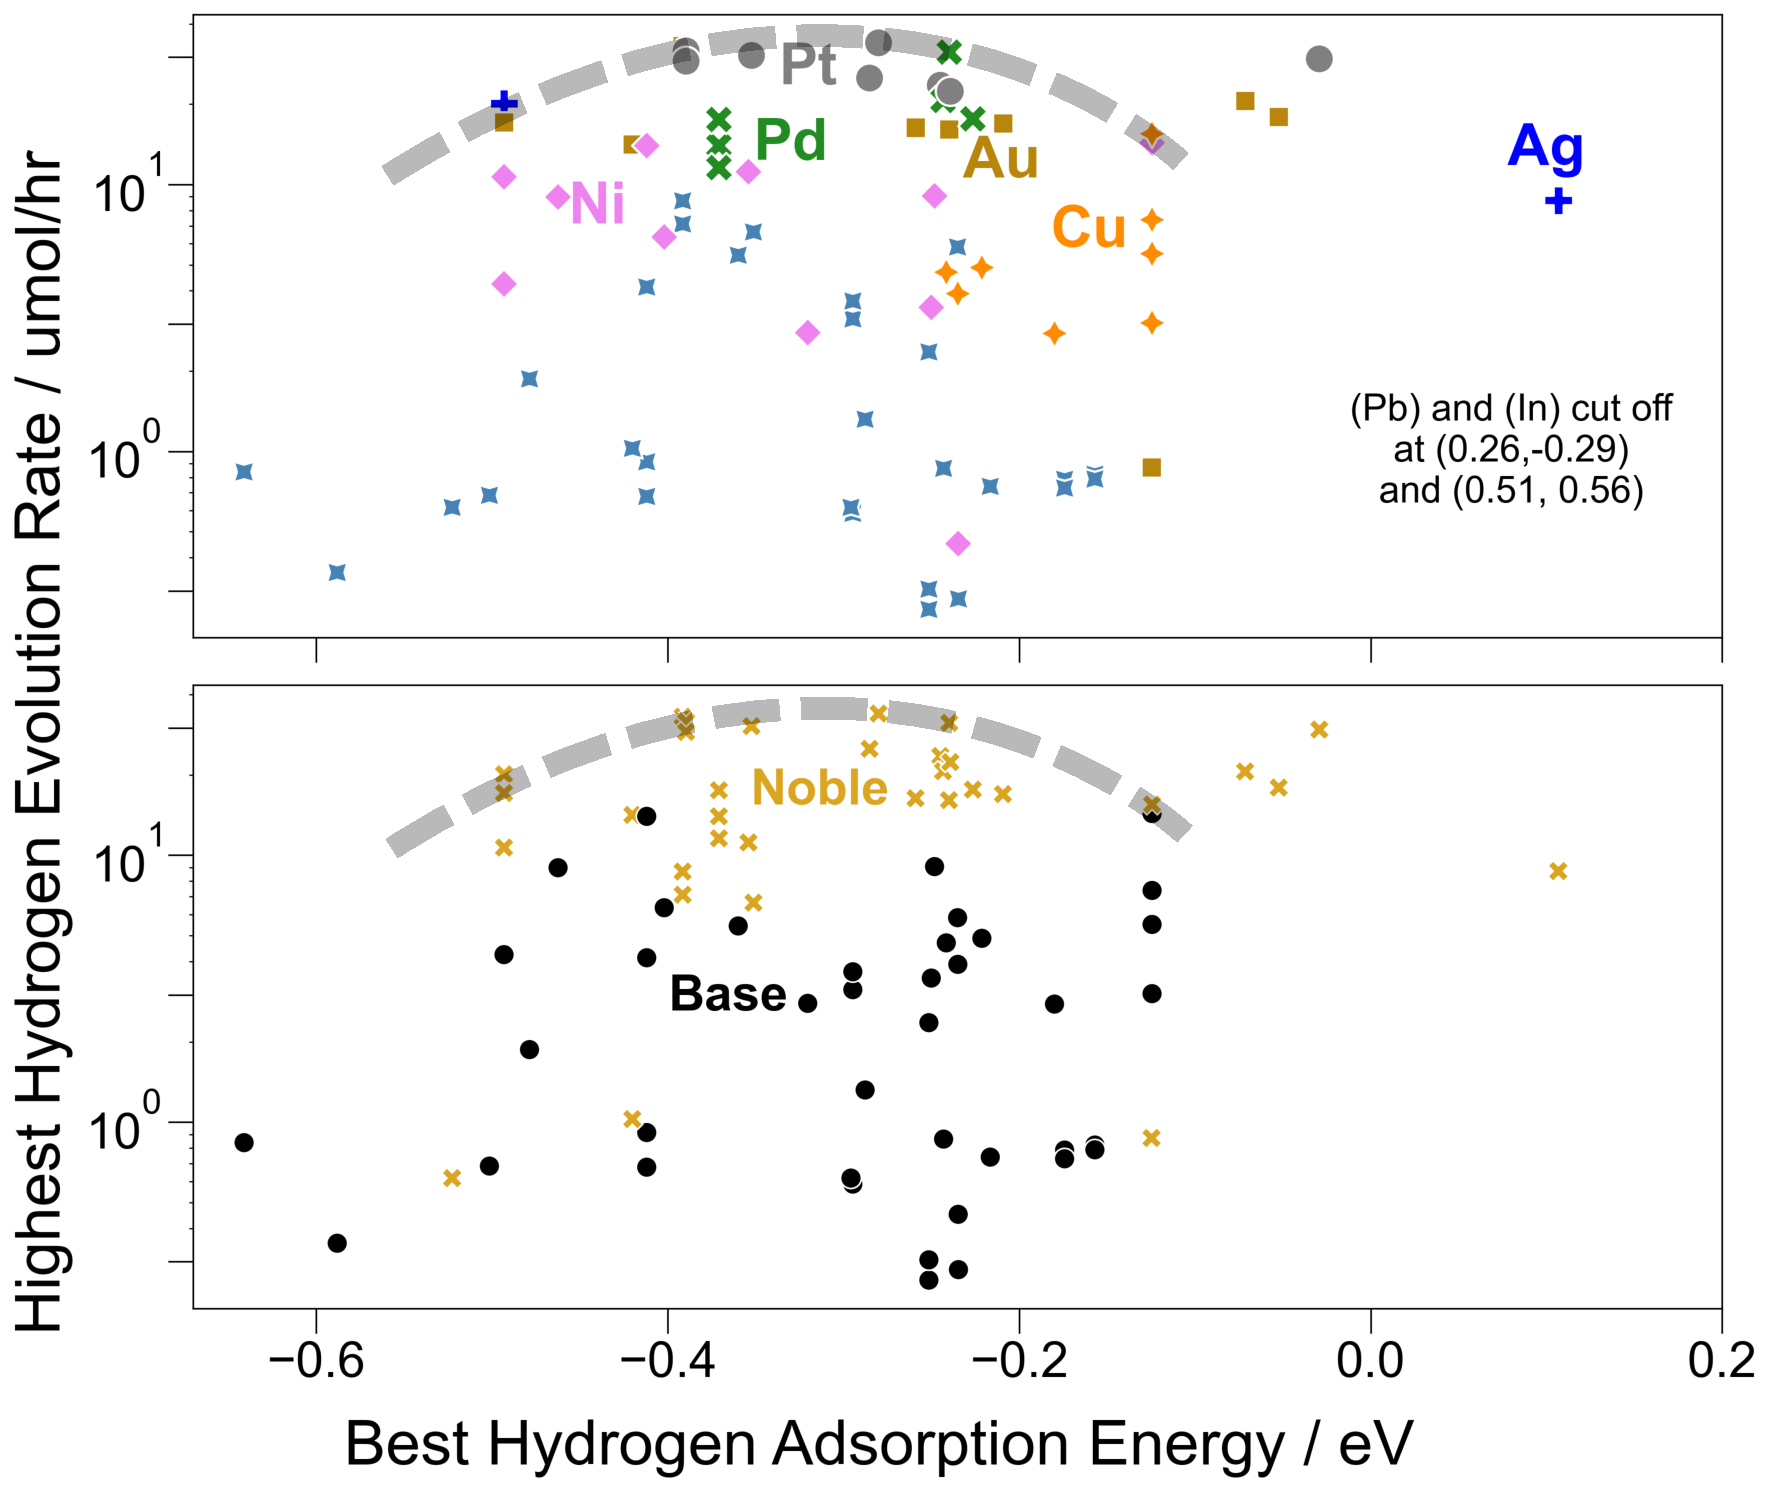
\includegraphics[width=0.7\textwidth]{figures/fig_4.pdf}
\caption{Volcano plots constructed by plotting the surface low-coverage hydrogen adsorption energy closest to the optimum (i.e. the surface minimum hydrogen adsorption energy closest to -0.24 eV) across all stable materials in for each metal combination against the highest experimental HER rate observed over all metal salt concentrations for that combination. A grey trend is drawn on as a guide for the eye. The three points to the right that lie above the trend contain Au and Ag, which are known to have improved hydrogen adsorption energies in nanoparticle form due to surface strain \cite{tran2018gold,campbell2009hydrogen}; the adsorption energies used in this work do not account for that effect. Note that the y-axis is not normalized by surface area, meaning that differences in absolute rates are affected by variations in the area of the total reactive interface. Materials with binding energies above 0.2 or below -0.65 eV (pure In, Pb, and Fe) were removed for clarity; none was experimentally active in any solvent condition. (a) This plot is colored by the metal in each bimetallic composition that had the highest pure activity: Pt (grey), Au (orange), Pd (green), Ni (pink), or Cu (orange). (b) This plot is colored by the presence (gold) or absence (black) of a noble metal. Across all solvent conditions, experiments containing at least one noble metal (shown in gold) tend to fall above the rest (black) at similar points on the x-axis.
}
\end{figure}

\begin{figure}[h]
\centering
    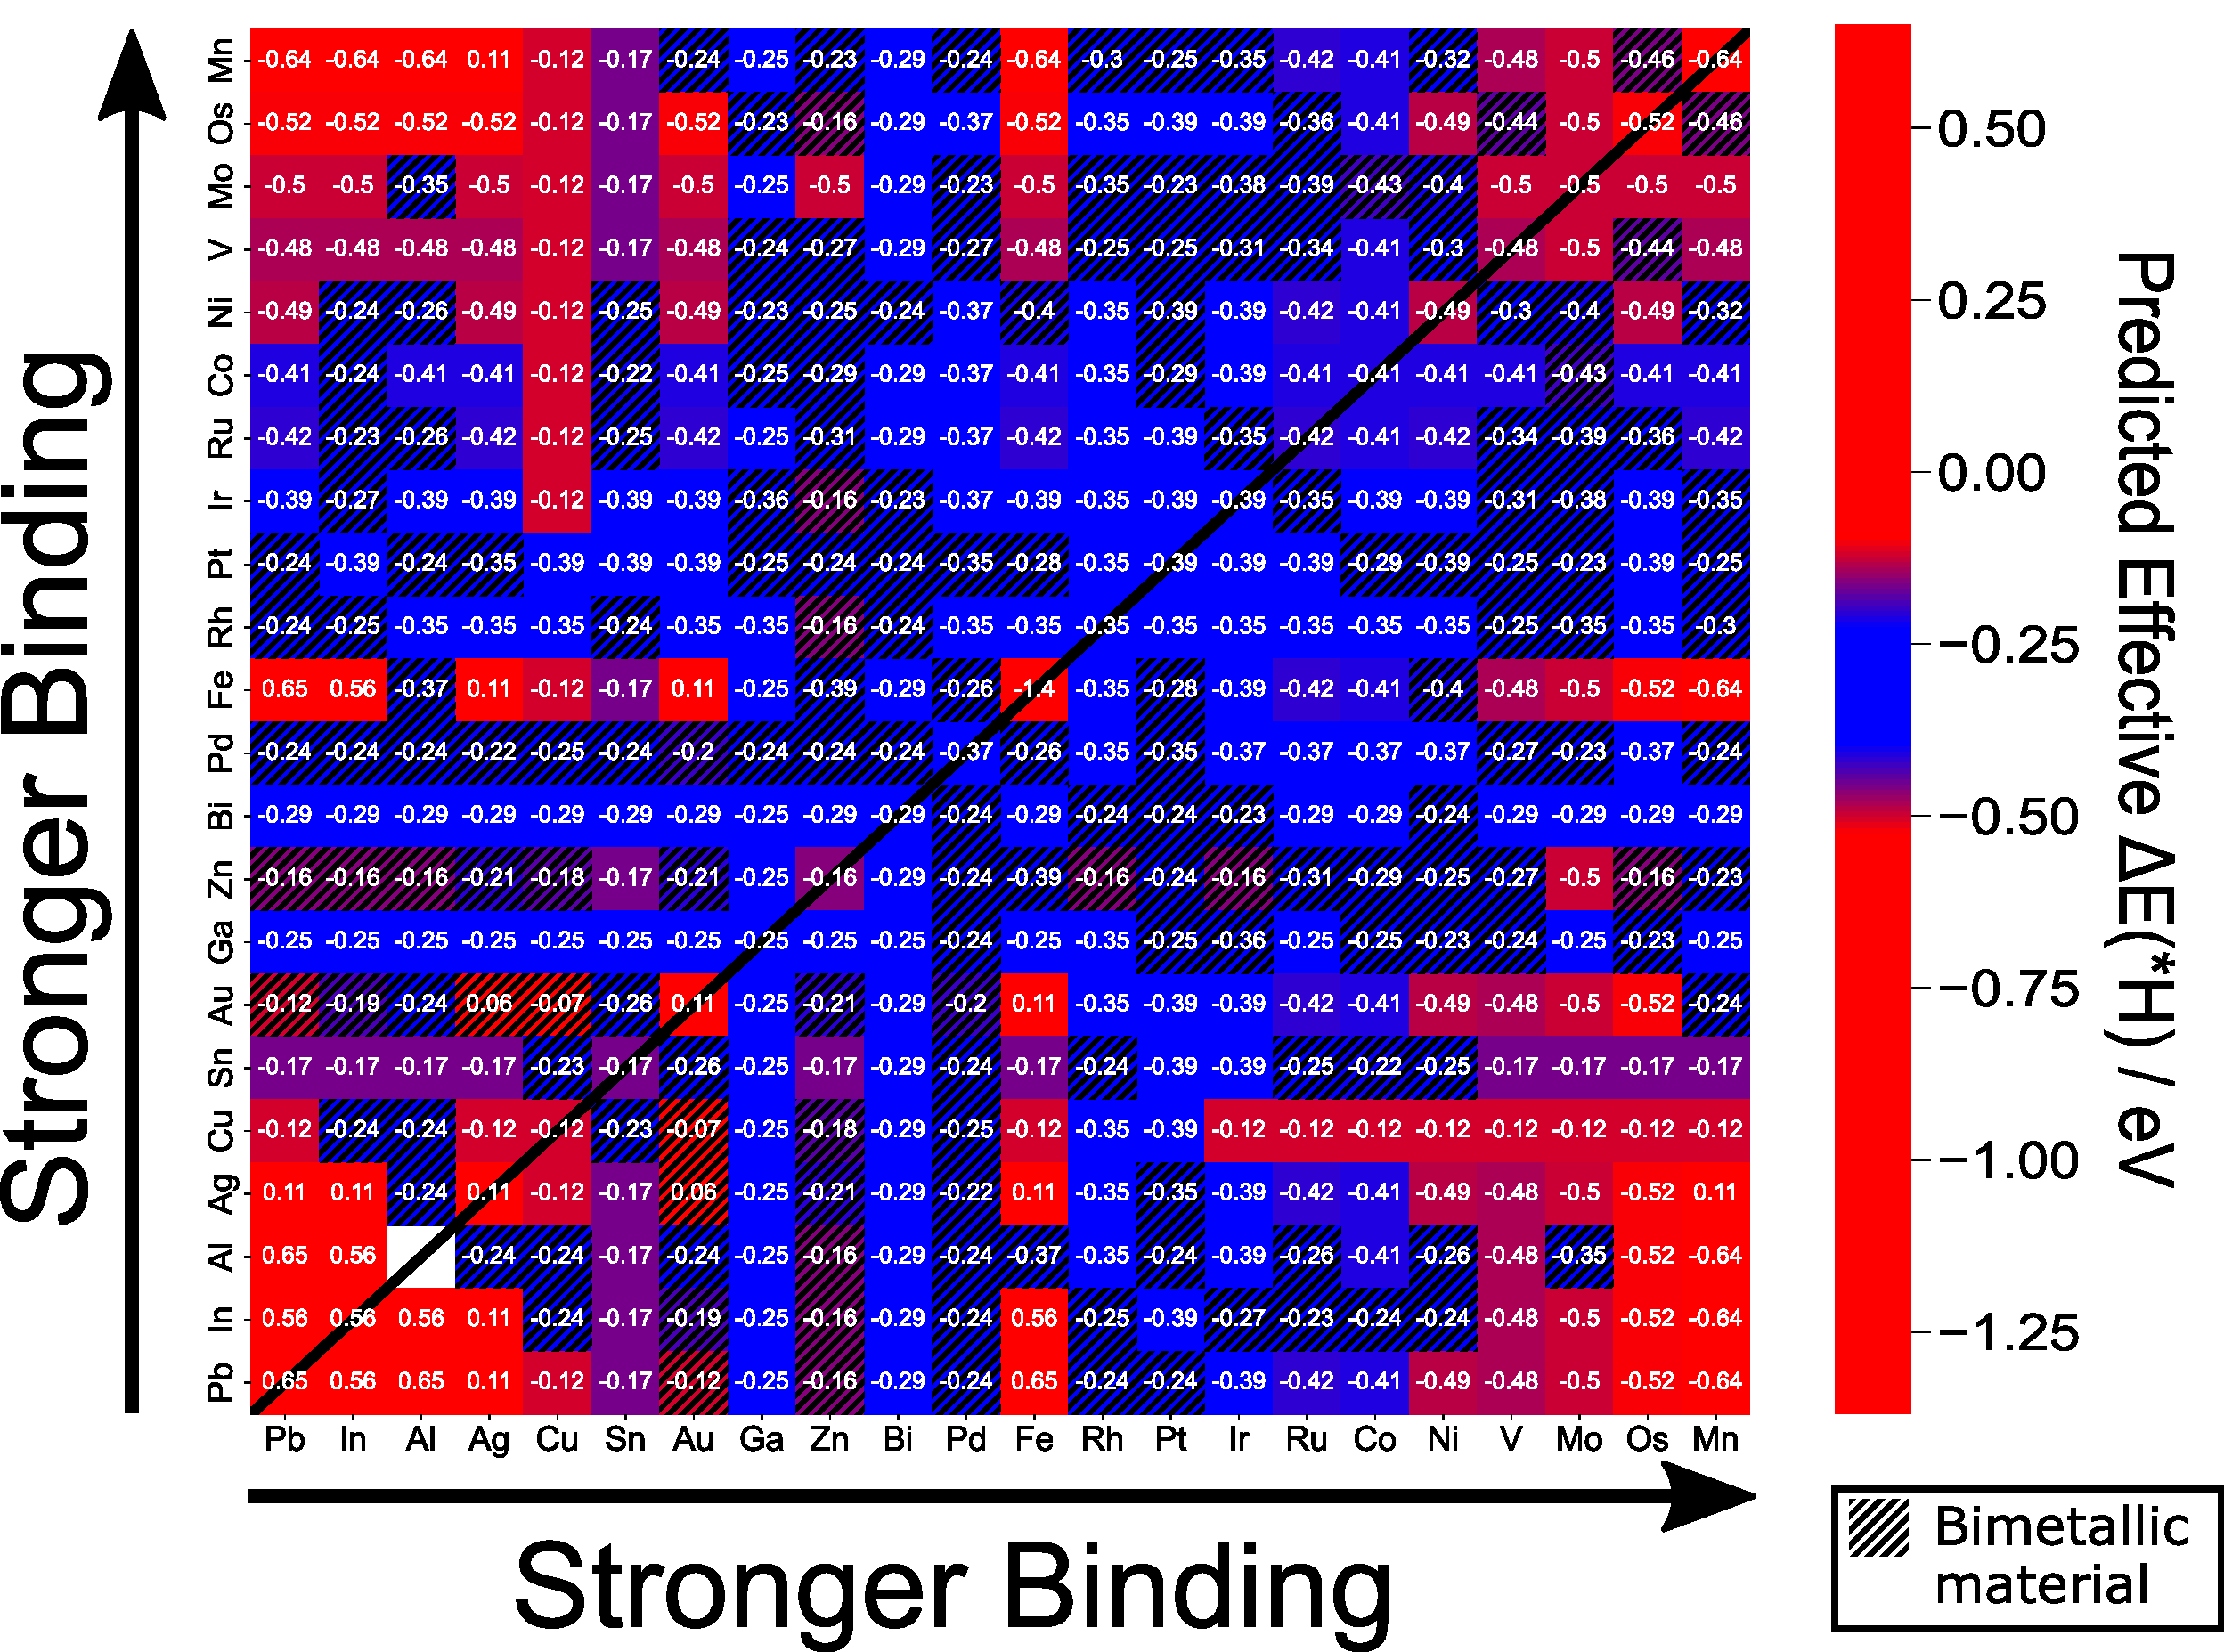
\includegraphics[width=0.8\textwidth]{figures/fig_5.pdf}
\caption{A grid plot of the predicted hydrogen binding energies of all combinations of metals involved in this work. Compositions where a bimetallic material is predicted to be the most active are hatched. Combinations predicted to have surfaces with favorable HER thermodynamics are shown in blue, demonstrating approximately a 50\% reduction in search space across all combinations or a 30\% reduction in combinations where a bimetallic material was expected to form (hatched). Pure aluminum was not predicted to form a metastable metal.
}
\end{figure}

With a view to this controversy, we observe that the most experimentally active chemical systems in our data contain materials with surfaces whose low-coverage binding energies are at or slightly stronger than thermodynamic neutrality ($-0.41 eV < \Delta E(H^*) < -0.23 eV$, see Fig. 4), whereas systems containing only thermodynamically unfavorable surfaces are less active, with the upper envelope of experimental activities relative to binding energies forming a volcano shape. This relationship is not perfect: a large number of chemical systems are predicted to express surfaces with favorable binding energies but are not very active experimentally. This observation is consistent with a physical picture in which aggregate reactivity is dominated by the most active surface present, but in some experiments this surface is deactivated or not present. One important caveat is that unlike in a Sabatier plot, plotted experimental activity is not normalized by surface area, meaning that data may underperform the Sabatier trend due to reduced surface area relative to the most active points. Additionally, this relationship is mediated by a substantial amount of noise in both the $x$- and $y$-axis (see Figures 1, 2). The full set of predictions generated using this method for all metal combinations can be seen in Figure 5.



\subsection{Noble Metals}\label{Section:Results/Noble}
Noble metals significantly outperformed base metals beyond what can be explained by adsorption thermodynamics alone (see Figure 4). In the volcano-type plot developed in this work, the HER activity for all experiments involving at least one noble metal was on average about an order of magnitude higher than activities from experiments using only base metals even if both systems expressed surfaces of equivalent binding energies (see Fig. 4). One possible explanation of this trend is that, although base metals may express thermodynamically active surfaces, these surfaces are less experimentally common than active surfaces on noble metals, either because particles are less likely to form or surfaces are deactivated. The latter prediction is supported by the experimental observation of oxides and sulfides on iron and nickle particles in a similar experimental system \cite{bhat2022accelerated}. Another compelling hypothesis is that 3d metals tend to have compact orbitals that cannot facilitate effective electron transfer \cite{quaino2014volcano}. However, the activity of weak-binding noble metals Au and Ag are also known to be significantly enhanced in nanoparticle form, with explanations for this trend including surface strain and surface cleanliness \cite{tran2018gold,campbell2009hydrogen,amin2014situ,merga2010naked,falsig2008trends}. Alternatively, the active surfaces on noble metals may be less easily poisoned, aggregated, or passivated: these effects were not considered in this work. Differences in nanoparticle stability may also have a substantial effect on activity trends \cite{simon2022ligand}.


\section{Conclusions}\label{Section:Conclusions}
To address challenges in connecting simple descriptors with complicated experimental catalysts, we developed an approach grounded in the Sabatier principle that aggregates adsorption energies over many active sites on different surfaces across a chemical system. We evaluated the usefulness of this relationship by comparing hydrogen adsorption energies predicted by machine-learned DFT surrogate models to hydrogen evolution reaction rates observed in a high-throughput experimental workflow outlined in previous work. In doing so, we discovered that thermodynamically favorable hydrogen adsorption sites are necessary for rapid hydrogen evolution but do not guarantee it, and we then outlined other factors, including poisoning, variation in nucleation and growth, surface expression, and strain effects, that may be modulating this relationship. This work extends the use of adsorption energy calculations as a useful catalyst screening tool to complex nanoparticle systems and increases demand for tools to understand other aspects of the catalytic process.

The model developed in this work extends catalyst design principles to large real-world datasets, representing an important step on the path to high-throughput in-the-loop materials discovery. Individual nanoparticle experiments can form materials with many compositions, structures, sizes, and surfaces that may show radically different catalyst activities, and we often cannot know beforehand what these distributions will look like. Materials discovery and design workflows need better strategies for modeling and learning these distributions automatically, which requires adapting and scaling well-known relationships as in this work. In particular, an understanding of the thermodynamic stability of materials and surfaces in different chemical environments will be important not only for understanding experimental observations but also in developing long-lasting catalysts for industrial use. Ultimately, as more advanced models are able to fit gaps in our current analytical understanding, they will ideally be integrated with experiments in closed-loop discovery workflows, accelerating and systematizing catalysis science.

The result in this work adds to a growing body of knowledge demonstrating that machine learning can be used to aid discovery by finding complex overlapping trends in large datasets. Because they make numerical predictions, such models can give insight into the scope and accuracy of current understanding in a way that qualitative explanations do not, and deviations from fitted models can guide scientists toward areas where new research is most needed. This work considers the ability of a single well-known trend to describe a complex dataset that poses many of the same problems as industrial design; the challenges in proving the presence of a well-established relationship in such a dataset point to the need for additional computational work to describe other physical phenomena in high throughput.


\section{Acknowledgement}
This research was supported by the Department of Energy, Office of Science, Office of Basic Sciences, Data Science for Knowledge Discovery for Chemical and Materials Research program, under award DE-SC0020392. The authors thank Kevin Tran for helpful discussions and Adeesh Kolluru for help using Open Catalyst Project resources and optimizing relaxations. E.M.L. was supported by the Steinbrenner Institute Graduate Fellowship and the ARCS Foundation Pittsburgh Chapter.

\section{Data and Code Availability}
Data used in this work as well as code for generating all figures is available at https://github.com/ulissigroup/DOE\_HER

%% The Appendices part is started with the command \appendix;
%% appendix sections are then done as normal sections

\bibliographystyle{elsarticle-num} 
\bibliography{bibliography}

\appendix
\documentclass[journal=accacs,manuscript=suppinfo]{achemso}
\SectionNumbersOn

\begin{document}

\tableofcontents

\section{Detailed Experimental Methods}
\subsection{Metal-cation precursors}
Metal-cation precursors used included: nickel(II) chloride anhydrous, Alfa Aesar B22085; potassium tetrachloroplatinate(II), Alfa Aesar 11048; ruthenium(III) chloride hydrate, Sigma-Aldrich 206229; molybdenum(III) chloride, Beantown Chemical 132345; potassium tetrachloropalladate(II), Beantown Chemical 129355; lead(II) chloride, Sigma-Aldrich 268690; tin(II) chloride dihydrate, Fisher Scientific S25578; silver trifluoromethanesulfonate, Alfa Aesar, 88722; aluminum trifluoromethanesulfonate, Oakwood Chemical, 003954; gold(III) chloride, Strem Chemical, 93-7907; bismuth(II) chloride, TCI, B3546; cobalt(II) chloride, Alfa Aesar, B22031; chromium(III) chloride hexahydrate, Strem Chemical, 93-2417; europium(III) chloride hexahydrate, Sigma-Aldrich, 203254; iron(II) chloride tetrahydrate, Sigma-Aldrich, 22,029-9; gallium nitrate hydrate, Alfa Aesar, 11150; indium(I) chloride, Alfa Aesar, 40033; iridium(III) chloride hydrate, J\&J Materials, 408828; lanthanum(III) chloride, Strem Chemical, 93-5708; lithium chloride, Acros, 199881000; manganese(II) chloride, Beantown Chemical, 137725; osmium(III) chloride hydrate, Acros, 318705000; rhodium(III) chloride hydrate, Thermo-Fischer, 900030512; vanadium(III) chloride, Strem Chemical, 23-4300; and zinc chloride, Alfa Aesar, 87900.

\section{Supplemental Figures}
\subsection{Volcano Plots in Various Media}
\begin{figure}[H]
\centering
    \includegraphics[width=0.9\textwidth]{figures/SI_figures/multimedia_comparison_volcano_fig_gemnet_SI.pdf}
\caption{Volcano plots constructed by plotting the low-coverage hydrogen binding energy of the most active surface (i.e. the surface with a low-coverage binding energy closest to -0.24 eV) against the highest \gls{HER} rate observed over all experiments for each chemical composition. Note that in all cases,  (a,b,) Volcano plots for (a) raw and (b) solvent-normalized experimental activities, colored by solvent: water and TEOA (blue), methanol (orange), and ethanol (green). Note that the $y$-axis is not normalized by surface area, meaning that variations in height or slope may be attributable to differences in the area of the total reactive interface. (c, d, e, f) Volcano plots for water/TEOA (c), methanol (d), ethanol (e), and solvent-normalized (f) experiments, colored by the most active pure component of each bimetallic composition: Pt (blue), Au (orange), Pd (green), or Cu (red).}
\label{fig:ComparisonSI}
\end{figure}

\subsection{Noble Metals by Solvent}
\begin{figure}[H]
\centering
    \includegraphics[width=0.7\textwidth]{figures/SI_figures/volcano_multimedia_by_noble_SI_gemnet.png}
\caption{Across all solvent conditions, experiments containing at least one noble metal were more experimentally active by approximately an order of magnitude. Significant positive outliers appear in the Sabatier trend if noble metals are excluded (annotated; note that in many cases the stablest crystal is not bimetallic)}
\label{fig:NobleSI}
\end{figure}
\subsection{Multimedia Experimental Activity Comparison}
\begin{figure}[H]
\centering
    \includegraphics[width=0.7\textwidth]{figures/SI_figures/experimental_variability_multimedia_SI.png}
\caption{(a,b,c) A comparison of the composition-averaged maximum observed rates of hydrogen evolution for each metal system across different reaction media. (d) The linear correlations of the composition-averaged maximum observed rates of hydrogen evolution for each metal system across different reaction media.}
\label{fig:ExperimentSI}
\end{figure}
\subsection{Gridplot Constructed Using Only System-specific Materials}
\begin{figure}[H]
\centering
    \includegraphics[width=0.7\textwidth]{figures/SI_figures/gridplot_fig_sparse_gemnet.pdf}
\caption{A grid plot of the hydrogen adsorption energy of the surface predicted to be most active. Only metal systems in which a unique compound is predicted to determine activity are shown, for example, Rh/Ir is now empty because the predicted active surface is on a material containing pure Ir.}
\label{fig:GridplotSI}
\end{figure}
\section{Data and Code Availability}
Data and code to run the analyses in this work and reproduce figures are available at https://github.com/Ulissigroup/HER\_Manuscript.

\end{document}

\end{document}
\endinput
%%
%% End of file `elsarticle-template-num.tex'.
